\chapter{进程与线程}

\section{进程与线程}

\subsection{进程的概念和特征}

    通常而言,在不同的认知角度上,对进程的定义是不同的,比较典型的定义为:

\begin{itemize}
    \item [1)] 进程是程序的一次执行过程
    \item [2)] 进程是一个程序及其数据在处理及上顺序执行时所发生的活动
    \item [3)] 进程是具有独立功能的程序在一个数据集合上运行的过程,是系统进行资源分配和调度的一个独立单位。
\end{itemize}

    当然的,在OS中,进程经过了抽象从而定义了一个重要的数据结构:进程控制块(Process Control Block,PCB)\footnote[1]{\emph{Linux中为task\_struct,定义在sche.h文件中}}。系统利用PCB来描述进程的基本情况和运行状态,进而控制和管理进程。\emph{相应地,由程序段、相关数据段和PCB三部分构成了进程实体(进程映像)。}

    注意:\emph{\color{red}PCB是进程存在的唯一标识}。

    \emph{进程映像可以被视为进程在内存中的静态表示,描述了进程的初始状态和资源分配情况。虽然进程映像在进程运行期间保持不变,但进程本身可能会发生动态的变化。}

    注意:\emph{\color{red}进程映像是静态的,进程则是动态的。}

    引入进程映像的概念后,又有了新的定义:\emph{进程是进程映像的运行过程,是系统进行资源分配和调度的一个独立单位。}

    进程是由多道程序的并发执行而引出的,其基本特征是对比单个程序的顺序执行提出的,也是对进程管理的基本要求:

\begin{itemize}
    \item [1)] 动态性。进程是程序的一次执行,{\color{red}动态性是进程最基本的特征}。
    \item [2)] 并发性。多个进程映像同存于内存中,能在一段时间内同时运行。{\color{red}并发性是进程的重要特征,也是OS的重要特征}。
    \item [3)] 独立性。进程映像是一个能独立运行、独立获得资源和独立接受调度的基本单位(此处暂时不考虑线程)。
    \item [4)] 异步性。由于进程的互相制约,使得进程各自独立、不可预知的向前推进。\emph{\color{red}异步性会导致执行的不可再现性,因此必须配置同步机制}。
\end{itemize}

\subsection{进程的状态与转换}

    进程在其生命周期内,会不断地发生状态变化。通常进程有五种状态,前三种是基本状态:

\begin{itemize}
    \item [1)] 运行态(Running)。进程正在CPU上运行。
    \item [2)] 就绪态(Runable)。进程获得了除处理机外的一切所需资源,\emph{通常处于就绪态的进程有多个,因此OS用就绪队列组织。}
    \item [3)] 阻塞态(Blocking/Waiting)。进程正在\emph{等待某一事件而暂停,通常处于阻塞态的进程有多个,因此OS用阻塞(等待)队列来组织,甚至可以根据阻塞原因设置多个阻塞队列。}
    \item [4)] 创建态(Creating)。进程正在被创建,未转到就绪态。
    \item [5)] 终止态(Exiting)。进程正在被释放或结束。
\end{itemize}

\begin{figure}[!htbp]
    \centering
    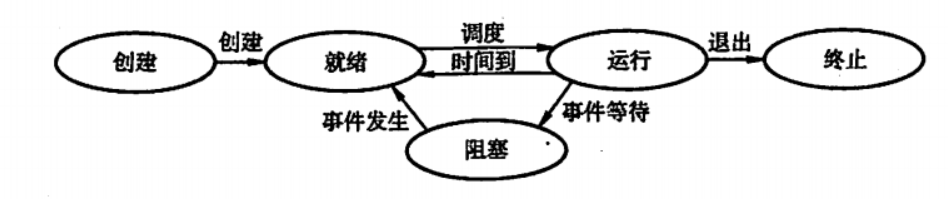
\includegraphics[width=0.8\textwidth]{image/chapter02/五种状态的转换.png}
    \caption{五种状态的转换}
\end{figure}

    值得注意的是:\emph{就绪态是指仅仅缺少处理机资源,也就是在就绪队列中还未到其处理的事件。而阻塞态是指,既缺乏处理机资源,又缺乏运行所需的必要资源(或事件发生)。}

    \emph{\color{red}一个进程从运行态变为阻塞态是主动的行为,从阻塞态变成就绪态是被动的行为。同时,就绪态不可能直接变为阻塞状态,因为变成阻塞必定是申请某种资源或事件发生,而这种情况之可能发生在运行时。}

\subsection{进程的组成}

    进程是一个独立的运行单位,也是OS进行资源分配和调度的基本单位。其由三个部分组成

\subsubsection{进程控制块}

    进程创建时,需要新建一个PCB常驻于内存中,PCB是进程存在的唯一标识,也是进程映射的一部分。

    \emph{在整个生命周期中,系统总是通过PCB对进程进行控制的,即系统唯有通过进程的PCB才能感知到该进程的存在。}

\begin{table*}[!htbp]
    \begin{center}
        \caption{PCB通常包含的内容}
        \begin{tabular}{c | c | c | c}
            \hline
            进程描述信息 & 进程控制和管理信息 & 资源分配清单 & 处理机相关信息 \\
            \hline
            进程标识符(PID) & 进程当前状态 & 代码段指针 & 通用寄存器值 \\
            \hline
            用户标识符(UID) & 进程优先级 & 数据段指针 & 地址寄存器值 \\
            \hline
            & 代码运行入口地址 & 堆栈指针 & 控制寄存器值 \\
            \hline
            & 程序外存地址 & 文件描述符 & 标志寄存器值 \\
            \hline
            & 进入内存时间 & 键盘 & 状态字 \\
            \hline
            & 处理机占用时间 & 鼠标 & \\
            \hline
            & 信号量使用 & & \\
            \hline
        \end{tabular}
    \end{center}
\end{table*}

\begin{itemize}
    \item [1)] 进程描述信息。\emph{\color{red}PID是进程的唯一标识符}。UID标识了进程所属的用户
    \item [2)] 进程控制和管理信息。
    \subitem 进程当前状态:描述进程的状态信息,作为调度的凭据
    \subitem 进程优先级:用于抢占机制
    \item [3)] 资源分配清单。用于说明内存地址空间或虚拟地址空间的状态,以及文件和I/O情况
    \item [4)] 处理机相关信息。用于保存进程的信息,当进程被切换时,必须将上下文信息保存在此处(线程就是为此的)。
\end{itemize}

    在OS中,为了满足各种情况,通常有:就绪队列,等待队列以及优先级队列,这三种队列都会保存在PCB中以供使用。

    特别的,一般而言还有另外一种组织方式:索引方式,将同一状态的进程组织在一张索引表内,然后通过索引表项指向PCB。

\subsubsection{程序段}

    程序段就是\emph{能够被进程调度程序调度到CPU执行的程序段代码。程序可能被多个进程共享。}

    代码段通常是只读的,意味着程序在运行时无法修改代码段中的指令。这是为了确保程序的逻辑和一致性。如果程序需要修改自身的指令,通常会使用特殊的技术,如自修改代码或动态代码生成。

    在计算机的内存中,代码段通常位于程序的虚拟地址空间的一个固定位置。操作系统负责将代码段加载到内存中,并为程序提供执行的环境和资源。

\subsubsection{数据段}

    一个进程的数据段,\emph{可以是进程对应的程序加工处理的原始数据,也可以是程序执行时产生的中间或最终结果。}

    进程的可变性,就主要体现在数据段中的变化。

\subsection{进程控制}

    进程控制的主要功能是对系统中的所有进程实施有效的控制,具有创建、删除、转换等原语。

\subsubsection{进程的创建}

    允许一个进程创建另一个进程。子进程可以继承父进程的所有资源。在OS中,系统调用的上层接口是fork(),而底层的原语接口是clone()。

    在OS中,终端用户登录系统、作业调度、系统提供服务、用户程序的应用请求等都会引起进程的创建:

\begin{itemize}
    \item [1)] 为新进程分配唯一的一个PID,并申请一个空白PCB。
    \item [2)] 为进程分配运行所需的各种资源。
    \item [3)] 初始化PCB,主要包括初始化标志信息、初始化CPU状态信息和初始化CPU控制信息,以及设置优先级
    \item [4)] 若进程就绪队列能够容纳,则并入就绪队列,等待被调度
\end{itemize}

\subsubsection{进程的终止}

    引起进程终止的事件主要有:正常结束;异常结束;外界干预这三种:

\begin{itemize}
    \item [1)] 根据被终止进程的标识符,检索出进程的PCB,从中读取进程状态
    \item [2)] 若被终止进程处于运行态,立即终止执行,并将处理机资源分配给其他任务
    \item [3)] 若该进程有子进程,则还应将子进程终止
    \item [4)] 将该进程的全部资源归还给父进程或OS
    \item [5)] 将该PCB从队列中移除
\end{itemize}

\subsubsection{进程的阻塞和唤醒}

    正在运行的任务,由于期待的事件尚未发生,进程便通过调用阻塞原语,使自身从运行态转变为阻塞状态。\emph{可见,阻塞态是一种进程的自身主动行为,因此只能处于在运行态的进程才可能转换为阻塞态}:

\begin{itemize}
    \item [1)] 找到将要被阻塞进程的标识号对应的PCB
    \item [2)] 若进程为运行态,则{\color{red}保护现场},将其转换为阻塞态,停止运行
    \item [3)] 将该PCB插入到对应事件的等待队列,将处理机资源调度给其他就绪任务
\end{itemize}

    当被阻塞进程所期待的事件发生时,由有关进程调用唤醒原语(Wakeup):

\begin{itemize}
    \item [1)] 在该事件的等待队列中找到响应的PCB
    \item [2)] 将其从等待队列中移除,并置为就绪态
    \item [3)] 把该PCB插入就绪队列,等待调度程序调度
\end{itemize}

    注意:\emph{阻塞和唤醒原语是一对作用相反的原语,因此需要成对使用。}

\subsubsection{进程的切换}

    进程的切换一般由于:当前进程时间片到;更高优先级任务到达;当前进程主动阻塞;当前进程终止等,这时就需要切换原语:

\begin{itemize}
    \item [1)] 将运行环境信息存入PCB
    \item [2)] PCB移入对应队列
    \item [3)] 选择另一个任务执行,更新PCB
    \item [4)] 根据PCB恢复新进程所需要的环境
\end{itemize}

    对于切换的原语,可以在内核中轻易的找到:

\begin{lstlisting}[language=C++]
#define switch_to(prev,next,last) \
asm volatile(SAVE_CONTEXT						    \
    "movq %%rsp,%P[threadrsp](%[prev])\n\t" /* save RSP */	  \
    "movq %P[threadrsp](%[next]),%%rsp\n\t" /* restore RSP */	  \
    "call __switch_to\n\t"					  \
    ".globl thread_return\n"					\
    "thread_return:\n\t"					    \
    "movq %%gs:%P[pda_pcurrent],%%rsi\n\t"			  \
    "movq %P[thread_info](%%rsi),%%r8\n\t"			  \
    "btr  %[tif_fork],%P[ti_flags](%%r8)\n\t"			  \
    "movq %%rax,%%rdi\n\t" 					  \
    "jc   ret_from_fork\n\t"					  \
    RESTORE_CONTEXT						    \
    : "=a" (last)					  	  \
    : [next] "S" (next), [prev] "D" (prev),			  \
    [threadrsp] "i" (offsetof(struct task_struct, thread.rsp)), \
    [ti_flags] "i" (offsetof(struct thread_info, flags)),\
    [tif_fork] "i" (TIF_FORK),			  \
    [thread_info] "i" (offsetof(struct task_struct, thread_info)), \
    [pda_pcurrent] "i" (offsetof(struct x8664_pda, pcurrent))   \
    : "memory", "cc" __EXTRA_CLOBBER)

struct task_struct *
__switch_to(struct task_struct *prev_p, struct task_struct *next_p)
\end{lstlisting}

\subsection{进程的通信}

    进程通信是指进程间的信息交换。PV操作是低级通信方式\footnote[1]{\emph{PV操作是一种用于进程同步的经典算法,用于解决进程之间的互斥和同步问题。PV操作通常与信号量(Semaphore)相关联。当进程需要访问共享资源时,执行P(wait)操作;当进程结束访问时,需要执行V(signal)操作。}},高级通信方式是指\emph{以较高的效率传输大量数据的通信方式}。

\subsubsection{共享存储}

    \emph{进程空间一般都是独立的,进程运行期间不能访问其他进程。}这是共享存储的前提条件,在通信的进程之间存在一块可以直接访问的共享空间,通过对该空间进行读写操作,实现进程间的消息互换。

\begin{figure}[!htbp]
    \centering
    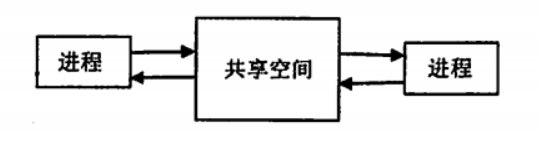
\includegraphics[width=0.6\textwidth]{image/chapter02/共享空间.png}
    \caption{共享存储}
\end{figure}

    为了实现共享存储,一般OS会提供上层接口以供使用。例如Linux中,提供了shm\_*等操作实现申请、撤销共享空间等操作,然后通过mmap将共享空间映射到进程自身的空间中。

    此处给出简单的示例:

\begin{lstlisting}[language=C++]
#include <stdio.h>
#include <stdlib.h>
#include <sys/mman.h>
#include <sys/stat.h>
#include <fcntl.h>
#include <unistd.h>
#include <sys/types.h>

int main() {
    const char* shm_name = "/my_shared_memory";
    int shm_fd = shm_open(shm_name, O_RDWR | O_CREAT, 0666);
    if (shm_fd == -1) {
        perror("shm_open");
        exit(1);
    }

    off_t size = 4096; // 共享内存的大小
    if (ftruncate(shm_fd, size) == -1) {
        perror("ftruncate");
        exit(1);
    }

    void* addr = mmap(NULL, size, PROT_READ | PROT_WRITE, MAP_SHARED, shm_fd, 0);
    if (addr == MAP_FAILED) {
        perror("mmap");
        exit(1);
    }

    // 现在可以通过addr指针来访问共享内存中的数据

    // 访问完成后,记得使用munmap函数解除映射
    if (munmap(addr, size) == -1) {
        perror("munmap");
        exit(1);
    }

    // 关闭共享内存文件描述符
    if (close(shm_fd) == -1) {
        perror("close");
        exit(1);
    }

    // 删除共享内存对象
    if (shm_unlink(shm_name) == -1) {
        perror("shm_unlink");
        exit(1);
    }

    return 0;
}
\end{lstlisting}

    对于共享存储而言,拥有两种方式:低级的共享是通过语言特性,例如全局的数据结构的共享,但是这样效率低、局限大;高级的共享就是通过这样实现一块存储区,速度快,局限小。

\subsubsection{消息传递}

    在消息传递系统中,进程间的数据交换以格式化的信息为单位。进程通过系统提供的发送/接收原语进行数据交换,\emph{这种方式隐藏了通信实现细节,使通信过程对用户透明,简化了通信程序的设计,是目前最广泛应用的机制。}

\begin{figure}[!htbp]
    \centering
    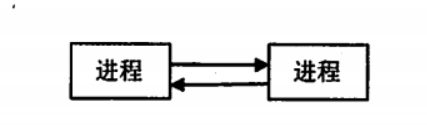
\includegraphics[width=0.4\textwidth]{image/chapter02/消息传递.png}
    \caption{消息传递}  
\end{figure}

\begin{itemize}
    \item [1)] 直接通信方式。发送进程直接把消息发送给接收进程,并将其挂在接收进程的消息缓冲队列上,接收进程从中获取消息。
    \item [2)] 间接通信方式。发送进程把消息发送到某个中间实体(类似于电子邮件的机制,是有一个邮件服务器的缓冲区),接收端从中间实体获取消息,该中间实体一般称为信箱。
\end{itemize}

\subsubsection{管道通信}

    \emph{在Linux中,管道是一种使用非常频繁的通信机制,本质上也是一种文件。}管道通信允许两个进程按生产-消费者模型进行通信,数据在管道中是FIFO的。管道的大小也是有规定的,一般为4KB(也就是说,是一个固定的缓冲区)。

    \emph{1. 管道只能采用半双工通信,某段时间内只能单向通信;但可以使用两个管道实现全双工通信。}

    \emph{2. 各进程需要互斥的读写管道。当管道写满时,写进程阻塞;当管道读空时,读进程堵塞。}

    \emph{3. 数据一旦被读取,一般情况下会消失。因此会出现争议:a). 一个管道允许多个写进程,一个读进程\footnote[1]{\emph{如果是答题,按照参考答案上的结果就是这样。如果从理解上来看,这种和后面一种的方式都是正确的。}}。b). 允许多个写进程,多个读进程,系统会让进程各自轮流读取\footnote[2]{\emph{Linux中的策略}}}。

    一个简单的示例,实现进程间互相通信:

\begin{lstlisting}[language=C++]
#include <stdio.h>
#include <stdlib.h>
#include <unistd.h>

int main() {
    int pipe1[2]; // 管道1,用于父进程向子进程发送数据
    int pipe2[2]; // 管道2,用于子进程向父进程发送数据

    if (pipe(pipe1) == -1 || pipe(pipe2) == -1) {
        perror("pipe");
        exit(1);
    }

    pid_t pid = fork();
    if (pid == -1) {
        perror("fork");
        exit(1);
    }

    if (pid == 0) {
        // 子进程
        close(pipe1[1]); // 关闭管道1的写端
        close(pipe2[0]); // 关闭管道2的读端

        char message[100];
        read(pipe1[0], message, sizeof(message)); // 从管道1读取数据
        printf("子进程收到消息:%s\n", message);

        const char* reply = "Hello, 父进程!";
        write(pipe2[1], reply, strlen(reply) + 1); // 向管道2写入数据

        close(pipe1[0]); // 关闭管道1的读端
        close(pipe2[1]); // 关闭管道2的写端
    } else {
        // 父进程
        close(pipe1[0]); // 关闭管道1的读端
        close(pipe2[1]); // 关闭管道2的写端

        const char* message = "Hello, 子进程!";
        write(pipe1[1], message, strlen(message) + 1); // 向管道1写入数据

        char reply[100];
        read(pipe2[0], reply, sizeof(reply)); // 从管道2读取数据
        printf("父进程收到消息:%s\n", reply);

        close(pipe1[1]); // 关闭管道1的写端
        close(pipe2[0]); // 关闭管道2的读端
    }

    return 0;
}
\end{lstlisting}

\subsection{线程和多线程模型}

\subsubsection{线程的基本概念}

    \emph{引入线程的目的是减少程序在并发执行时所付出的时空开销,提高OS的并发性能。}

    线程最为直接的理解就是“轻量级进程”,\emph{是一个基本的CPU执行单元,也是程序执行流的最小单元。}线程是进程的一个实体,\emph{{\color{red}是被OS独立调度和分派的基本单位}(引入线程后,进程就不再是调度的基本单位了),线程不拥有系统资源,但可以与同属进程的其他线程共享所拥有的全部资源。}

    那么,现在重新定义:\emph{进程是只作为除CPU外的系统资源的分配单元,线程作为处理机的分配单元。}

\subsubsection{线程与进程的比较}

\begin{itemize}
    \item [1)] 调度
    \subitem 引入线程后,\emph{线程是独立调度的基本单位},线程切换的代价远小于进程,同时,在同一进程中的不同线程切换,不需要切换进程。
    \item [2)] 并发性
    \subitem 不仅进程能够并发,线程也是能够并发的,准确来说,线程就是为此而生的
    \item [3)] 拥有资源
    \subitem \emph{进程是系统中拥有资源的基本单位,线程不拥有系统资源,但能够访问所属进程的资源(主要表现在,同一进程中的所有线程具有相同的地址空间)}
    \item [4)] 独立性
    \subitem \emph{每个进程都拥有独立的地址空间和资源,除了共享的全局变量;而同一进程的所属线程间,共享进程的地址空间和资源。}
    \item [5)] 系统开销
    \subitem 显然,线程的各种开销明显小于进程
    \item [6)] 支持多处理机系统
\end{itemize}

\subsubsection{线程的状态和转换}

    与进程类似,各线程间因为并发的原因也存在共享资源和相互合作的制约关系:

\begin{figure}[!htbp]
    \centering
    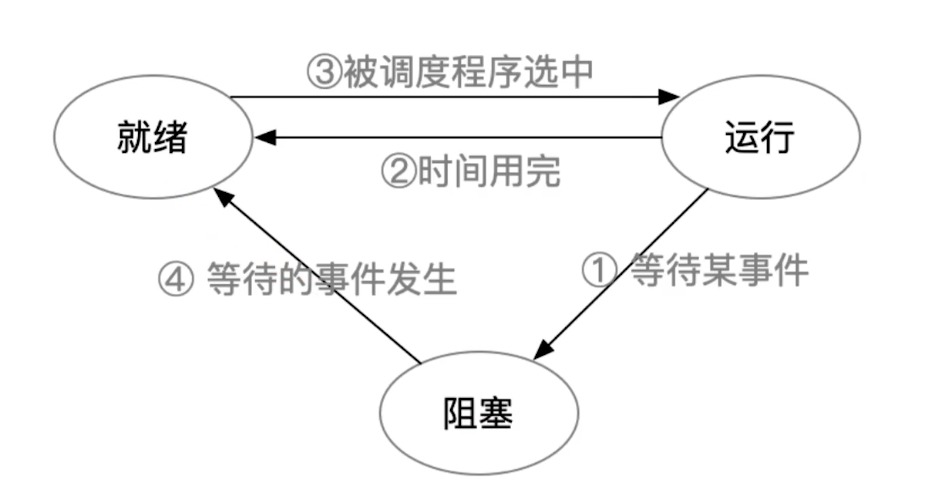
\includegraphics[width=0.6\textwidth]{image/chapter02/线程的状态与转换.png}
    \caption{线程的状态与转换}
\end{figure}

\subsubsection{线程的组织与控制}

    与进程类似,OS也为线程配置了一个线程控制块TCB,用于记录控制和管理线程的信息。

\begin{figure}[!htbp]
    \centering
    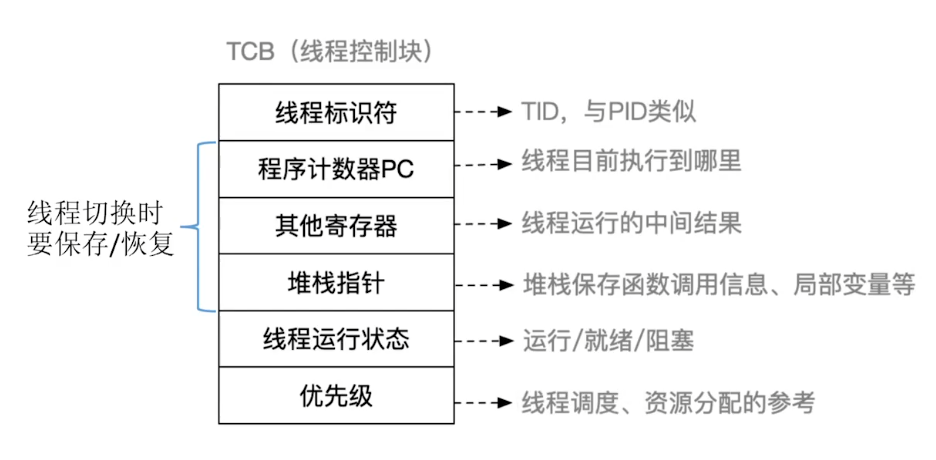
\includegraphics[width=0.6\textwidth]{image/chapter02/TCB.png}
    \caption{TCB}
\end{figure}

    同一进程中所有线程都完全共享进程的空间与资源,一个线程能够读写甚至删除另一个线程的堆栈。同时,线程的创建和终止也和进程类似,不过在删除时,必须考虑进程的因素,从而选择是否释放资源。

\subsubsection{线程的实现方式}

    线程的实现可以分为两类:用户级线程(User-Level Thread,ULT)和内核级线程(Kernel-Level Thread)

\paragraph{用户级线程}

    \emph{在用户级线程中,有关线程管理的所有工作都是由应用程序在用户态完成的,{\color{red}内核根本意识不到线程的存在}。}因此,对于设置了ULT的系统,其调度实际上还是以进程为单位的。

    这种方式的优点在于:

    \emph{1. 线程切换不需要进入到内核态,节省了切换的开销。}

    \emph{2. 调度算法是进程专用的,不同进程可根据自身需求,为自己的线程选择不同的调度算法。}

    \emph{3. 用户级线程的实现与OS无关,对线程管理的代码属于用户程序的一部分}

    而缺点在于:

    \emph{1. 系统调用的阻塞不仅会导致该进程被阻塞,且进程内的所有线程都会被阻塞}

    \emph{2. 严重降低了处理效率,不能发挥多处理机的优势}

\paragraph{内核级线程}

    内核级线程是由内核支持的,线程管理的工作在内核空间中实现。因此内核为每个线程设置了TCB,\emph{\color{red}内核能够对内核级线程进行感知。}

    这种方式的优点在于:

    \emph{1. 发挥了多处理机的优势,能够同时调度同一进程中的多个线程}

    \emph{2. 如果进程中的一个线程阻塞,那么可以对另外一个线程进行调度}

    \emph{3. 内核支持线程具有小的数据结构和堆栈,切换较快,开销较小}

    \emph{4. 内核本身也提供多线程技术,提高系统的执行效率}

    而缺点在于:

    \emph{同一进程中的线程切换,需要转换到内核态,系统开销较大。}

\paragraph{ULT \& KLT}

    ULT和KLT的组合能够使得结合各自的优点并克服各自的不足。支持多个内核级线程的建立、调度和管理,同时允许用户级线程的使用,能够使得线程阻塞但不会导致其他线程阻塞。

\begin{figure}[!htbp]
    \centering
    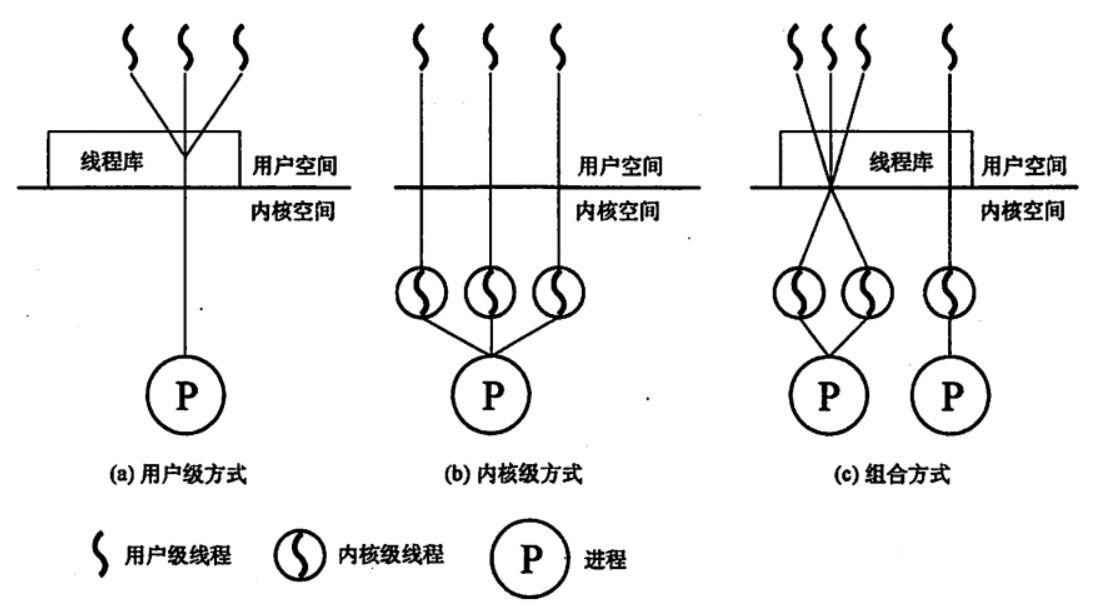
\includegraphics[width=0.8\textwidth]{image/chapter02/用户级线程和内核级线程.png}
    \caption{用户级线程和内核级线程}
\end{figure}

\subsubsection{多线程模型}

    基于有些系统同时支持用户线程和内核线程,因此就会产生不同的多线程模型:

\paragraph{多对一模型}

    将多个用户级线程映射到一个内核级线程(一般来说,多对一就是特指一个内核级线程),这些用户级线程通常属于一个进程。

    优点:线程管理在用户空间进行,效率较高

    缺点:一个线程发生阻塞,那么整个进程都会阻塞;且任何时刻只能由一个线程访问内核

\paragraph{一对一模型}

    每个用户级线程映射到一个内核级线程

    优点:当一个线程被阻塞后,允许调度另一个线程,并发能力较强

    缺点:每创建一个用户线程,都需要一个内核线程,开销过大

\paragraph{多对多模型}

    将n个用户级线程映射到m个内核级线程,要求$n \geq m$

    特点:既克服了多对一模型并发度不高的缺点,又克服了一对一模型开销过大的问题。

\begin{figure}[!htbp]
    \centering
    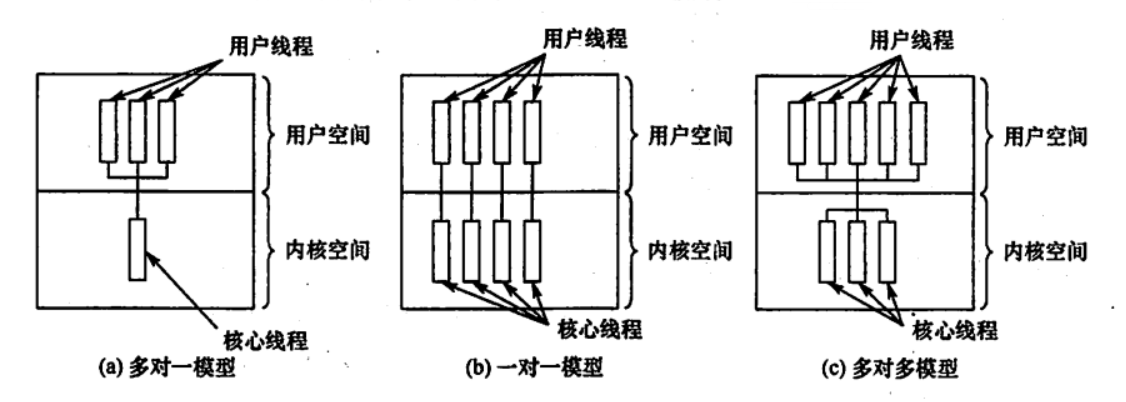
\includegraphics[width=0.8\textwidth]{image/chapter02/多线程模型.png}
    \caption{多线程模型}
\end{figure}

